\chapter{Design of Module \textit{userprog}}


\section{Process Termination Messages \& Argument passing}

    \subsection{Initial Functionality}

	At the beginning of this project ... .

    \subsection{Data Structures and Functions}

    \begin{lstlisting}

      "In thread.h :"
	
	struct thread {
	    /* The process id to which the thread
	       belongs to. */
	       int pid;
	};

	/* comments */
	variable definition;

	/* comments */
	function definition;

    \end{lstlisting}


    \subsection{Functionality}

	Function x works like this ... : (picture with sequence diagram or algorithm. See commented examples for including images or describing algorithms below)

    %\begin{figure}[h]
    %	\centering
    %	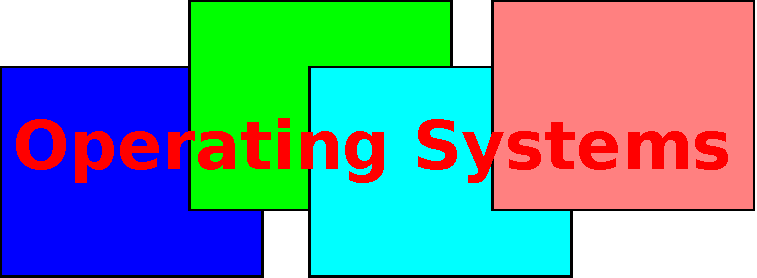
\includegraphics[width=0.5\textwidth]{figures/sample-image.pdf}
    %	\caption{Sample image}
    %	\label{fig:sample-image}
    %\end{figure}


    %Here you have a pseudo-code description of an algorithm taken fom \\ \href{http://en.wikibooks.org/wiki/LaTeX/Algorithms\_and\_Pseudocode\#Typesetting\_using\_the\_program\_package}{http://en.wikibooks.org/wiki/LaTeX}. It uses the \textit{program} package. Alternatively, you can use \textit{algorithmic} or \textit{algorithm2e} packages. 

    %\begin{program}
    %\mbox{Example of a pseudo-code algorithm description:}
    %\BEGIN %
    %  \FOR i:=1 \TO 10 \STEP 1 \DO
    %     |expt|(2,i); \\ |newline|() \OD %
    %\rcomment{This text will be set flush to the right margin}
    %\WHERE
    %\PROC |expt|(x,n) \BODY
    %          z:=1;
    %          \DO \IF n=0 \THEN \EXIT \FI;
    %             \DO \IF |odd|(n) \THEN \EXIT \FI;
    %\COMMENT{This is a comment statement};
    %                n:=n/2; x:=x*x \OD;
    %             \{ n>0 \};
    %             n:=n-1; z:=z*x \OD;
    %          |print|(z) \ENDPROC
    %\END
    %\end{program}


    \subsection{Design Decisions}

	This solution has the advantage that ... 

	On the other hand it is not so good that ... . 

	A better solution would be ... . 

	However, this solution is better than ...

    \subsection{Tests}

    \textbf{name of the test}\\
    \textit{Source:} path/to/test.c\\
    \textit{Purpose:} What does it check?\\
    \textit{Description:} Short description.
    \textit{Solution:(if necessary)} Here, if what the test does is something that was not explicitly asked in the requirements, it would be good to say that we already treat that situation and where. If it's something that should be solved only by the implementation of the requirements you can say: Solved by requirements fulfillment.
    
\section{System calls}

    \subsection{Initial Functionality}

	At the beginning of this project, pintOS does not provide the posibility of running any kind of user programs, much less make system calls from them. Moreover, there is no data structure to support processes. Our purpose is to implement the data structures required to support processes, as well as making various system calls.

    \subsection{Data Structures and Functions}

    \begin{lstlisting}

    "In process.h :"
      
      /* maximum number of processes running at the same 
      time. May need some adjustments. */
      #define MAX_PROCESSES 1024

      /* possible states of a process. 
	  ALIVE  is a process that has still not finished 
		 it's execution. 
	  KILLED is a process killed by the kernel.
	  DEAD 	 is a process that was killed at user's 
		 request by calling exit. */
      enum process_status_type {ALIVE, KILLED, DEAD}

      struct process {
	  /* pid (process id) of this process's parent */
	  int ppid;				
	  
	  /* status of the process: one of ALIVE, KILLED, 
	     DEAD. */
	  process_status_type status;
      
	  /* the code returned by the process at exit */
	  int exit_code;

	  /* The thread that is waiting after this thread. */
	  struct thread* waiting_thread;

	  /* In construction ... Come back soon! */
	  void *etc;
      };

      "In process.c: "

      /* The processes table */
      static struct processes_table[MAX_PROCESSES];

      "In userprog/syscalls.h: (kernel side)"
      
      /* synchronisation lock in order to execute
	 only one syscall at a time */
      static struct lock syscall_lock;

      /* Reads a byte at user virtual address UADDR.
	UADDR must be below PHYS_BASE.
	Returns the byte value if successful, -1 if a 
	segfault occurred. 
	PROBLEM!!! WHAT HAPPENS IF BYTE AT UADDR IS -1?*/
      static int get_user (const uint8_t *uaddr);

      /* Writes BYTE to user address UDST.
	 UDST must be below PHYS_BASE.
	 Returns true if successful, false if a segfault 
	 occurred. */
      static bool put_user (uint8_t *udst, uint8_t byte);

    \end{lstlisting}


    \subsection{Functionality}

	Function x works like this ... : (picture with sequence diagram or algorithm. See commented examples for including images or describing algorithms below)

	\textbf{Exit sycall}
	  \begin{program}
	    syscall\_lock.aquire();
	    proc\_crt = processes\_table[current\_thread.pid];
	    proc\_crt.exit\_code = status;
	    thread\_exit();
	    proc\_crt.status = DEAD;
	    \IF proc\_crt.waiting\_thread != NULL 
	      \THEN sycall\_lock.release(); 
	      thread\_unblock(proc\_crt.waiting_thread); 
	    \FI
	  \end{program}


    \subsubsection{wait}
    \begin{lstlisting}

    //in thread.h
    struct thread_t {
        ...
        pid_t process_id;
        ...
    };

    //in process.h
    ...
    struct process_t {
        pid_t id;
        pid_t parent_id;
        pstatus_t status;        
        int exit_code;
    };
    ...
    typedef struct process_t process_t;

    // we need a table with all processes, a hash table will do fine, standard C array too.

    int
    process_wait (pid_t child_pid UNUSED) 
    {
        lock_aquire(&process_wait_lock);
        if(child_tid does not exist) //we test if child_tid is in the table.
            return -1;

        if(get_process().id != get_process(child_pid).parent_id)
            return -1;

        int exit_code;

        if(get_process(child_pid).status == KILLED) {
            exit_code = -1;
            
        }
        else if(get_process(child_pid).status == DEAD) {
            exit_code = get_process(child_pid).exit_code;            
        }
        else if(get_process(child_pid).status == RUNNING) {
            thread_block(); // or some sort of busy interruptible waiting.
            // or we can set the exit code to a value and do the busy waiting in userspace.
            // the problem with that approach is that the user can set the same code and then will generate a freeze. We could solve this by returning additional information

            exit_code = get_process(child_pid).exit_code;
        }

        clean_child(child_pid);
        return exit_code;
    }

    
    \end{lstlisting}



    %\begin{figure}[h]
    %	\centering
    %	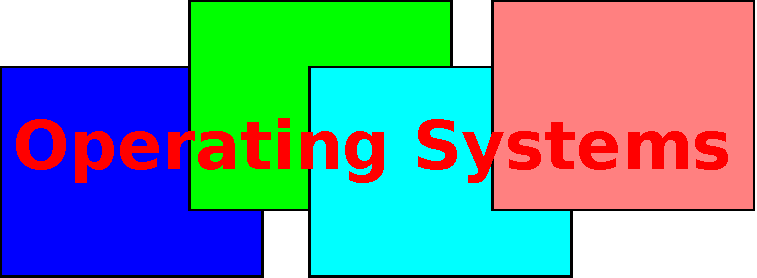
\includegraphics[width=0.5\textwidth]{figures/sample-image.pdf}
    %	\caption{Sample image}
    %	\label{fig:sample-image}
    %\end{figure}


    %Here you have a pseudo-code description of an algorithm taken fom \\ \href{http://en.wikibooks.org/wiki/LaTeX/Algorithms\_and\_Pseudocode\#Typesetting\_using\_the\_program\_package}{http://en.wikibooks.org/wiki/LaTeX}. It uses the \textit{program} package. Alternatively, you can use \textit{algorithmic} or \textit{algorithm2e} packages. 

    %\begin{program}
    %\mbox{Example of a pseudo-code algorithm description:}
    %\BEGIN %
    %  \FOR i:=1 \TO 10 \STEP 1 \DO
    %     |expt|(2,i); \\ |newline|() \OD %
    %\rcomment{This text will be set flush to the right margin}
    %\WHERE
    %\PROC |expt|(x,n) \BODY
    %          z:=1;
    %          \DO \IF n=0 \THEN \EXIT \FI;
    %             \DO \IF |odd|(n) \THEN \EXIT \FI;
    %\COMMENT{This is a comment statement};
    %                n:=n/2; x:=x*x \OD;
    %             \{ n>0 \};
    %             n:=n-1; z:=z*x \OD;
    %          |print|(z) \ENDPROC
    %\END
    %\end{program}


    \subsection{Design Decisions}

	This solution has the advantage that ... 

	On the other hand it is not so good that ... . 

	A better solution would be ... . 

	However, this solution is better than ...

    \subsection{Tests}

    \textbf{name of the test}\\
    \textit{Source:} path/to/test.c\\
    \textit{Purpose:} What does it check?\\
    \textit{Description:} Short description.
    \textit{Solution:(if necessary)} Here, if what the test does is something that was not explicitly asked in the requirements, it would be good to say that we already treat that situation and where. If it's something that should be solved only by the implementation of the requirements you can say: Solved by requirements fulfillment.
	

\section{Denying writes to executables}

     \subsection{Initial Functionality}

	At the beginning of this project ... .

    \subsection{Data Structures and Functions}

    \begin{lstlisting}

      "In ... :"
	
	struct structure_def {
	    type field;
	};

	/* comments */
	variable definition;

	/* comments */
	function definition;

    \end{lstlisting}


    \subsection{Functionality}

	Function x works like this ... : (picture with sequence diagram or algorithm. See commented examples for including images or describing algorithms below)

    %\begin{figure}[h]
    %	\centering
    %	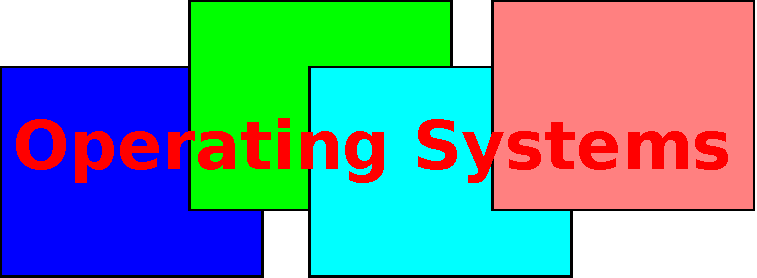
\includegraphics[width=0.5\textwidth]{figures/sample-image.pdf}
    %	\caption{Sample image}
    %	\label{fig:sample-image}
    %\end{figure}


    %Here you have a pseudo-code description of an algorithm taken fom \\ \href{http://en.wikibooks.org/wiki/LaTeX/Algorithms\_and\_Pseudocode\#Typesetting\_using\_the\_program\_package}{http://en.wikibooks.org/wiki/LaTeX}. It uses the \textit{program} package. Alternatively, you can use \textit{algorithmic} or \textit{algorithm2e} packages. 

    %\begin{program}
    %\mbox{Example of a pseudo-code algorithm description:}
    %\BEGIN %
    %  \FOR i:=1 \TO 10 \STEP 1 \DO
    %     |expt|(2,i); \\ |newline|() \OD %
    %\rcomment{This text will be set flush to the right margin}
    %\WHERE
    %\PROC |expt|(x,n) \BODY
    %          z:=1;
    %          \DO \IF n=0 \THEN \EXIT \FI;
    %             \DO \IF |odd|(n) \THEN \EXIT \FI;
    %\COMMENT{This is a comment statement};
    %                n:=n/2; x:=x*x \OD;
    %             \{ n>0 \};
    %             n:=n-1; z:=z*x \OD;
    %          |print|(z) \ENDPROC
    %\END
    %\end{program}


    \subsection{Design Decisions}

	This solution has the advantage that ... 

	On the other hand it is not so good that ... . 

	A better solution would be ... . 

	However, this solution is better than ...

    \subsection{Tests}

    \textbf{name of the test}\\
    \textit{Source:} path/to/test.c\\
    \textit{Purpose:} What does it check?\\
    \textit{Description:} Short description.
    \textit{Solution:(if necessary)} Here, if what the test does is something that was not explicitly asked in the requirements, it would be good to say that we already treat that situation and where. If it's something that should be solved only by the implementation of the requirements you can say: Solved by requirements fulfillment.
